\large
	\def\imbcircle{(-210:2) circle (2.725cm)}
	\def\dscircle{(-330:2) circle (2.725cm)}
	\def\mdcircle{(-90:2) circle (2.725cm)}

	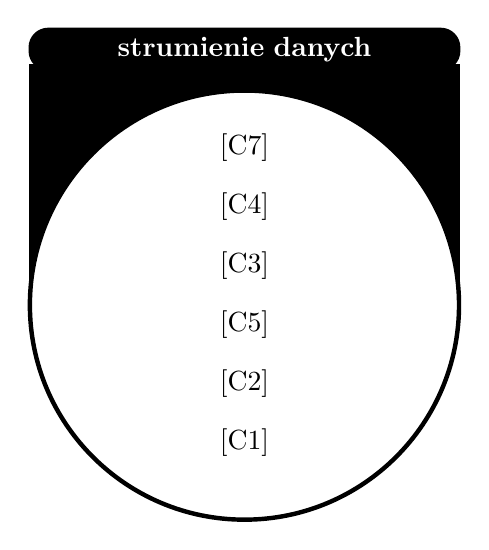
\begin{tikzpicture}
      	
      	\node[fill=black,rotate=0, text width=5.25cm, text height=2.9cm] at (90:-.5) {};
		\node[color=white,fill=black,rotate=0,rounded corners=.25cm, text width=5.25cm, align=center] at (90:1.25) {\bfseries \textsc{strumienie danych}};
      	
      	\draw[fill=white] \mdcircle;
      	\draw[ultra thick] \mdcircle;
      	
      	% 10 9 11 
      	% MD
      	\node at (-90:0) {[C7]};
      	\node at (-90:.75) {[C4]};    
      	\node at (-90:1.5) {[C3]};    
      	\node at (-90:2.25) {[C5]};    
      	\node at (-90:3) {[C2]};    
      	\node at (-90:3.75) {[C1]};
	\end{tikzpicture}